% ************ Chapter 2 ************
\chapter{Contexto} 
\label{cap:2}
\section{Processo de reciclagem}
O espaço físico da fábrica esta divido em duas partes: a primeira onde fica o armazém e onde é recepcionado a materia-prima e um segundo espaço onde existe uma máquina que corta o corpo de plástico do círio, tendo apenas de o colaborador a seguir que abrir o corpo e separar a cera do plástico. A alimentar esta máquina está um operador que recebe o corpo do círio sem nenhum elemento metálico, tendo apenas que colocar o círio devidamente alinhado. Alguns círios, devido à sua forma, não podem ser processado nessa mesma máquina, tornando-se necessário que exista um ponto de separação manual. Terminada a separação, a cera é levada para o forno. Quando a cera termina de ser derretida é enformada e colocada num espaço de ar condicionado para arrefecer e solidificar. Normalmente este processo é feito ao fim do dia e durante a noite para poder aproveitar a baixa de temperatura ambiental.

%\begin{figure}[H] 
%	\begin{center}
%		Requires \usepackage{graphicx}
%		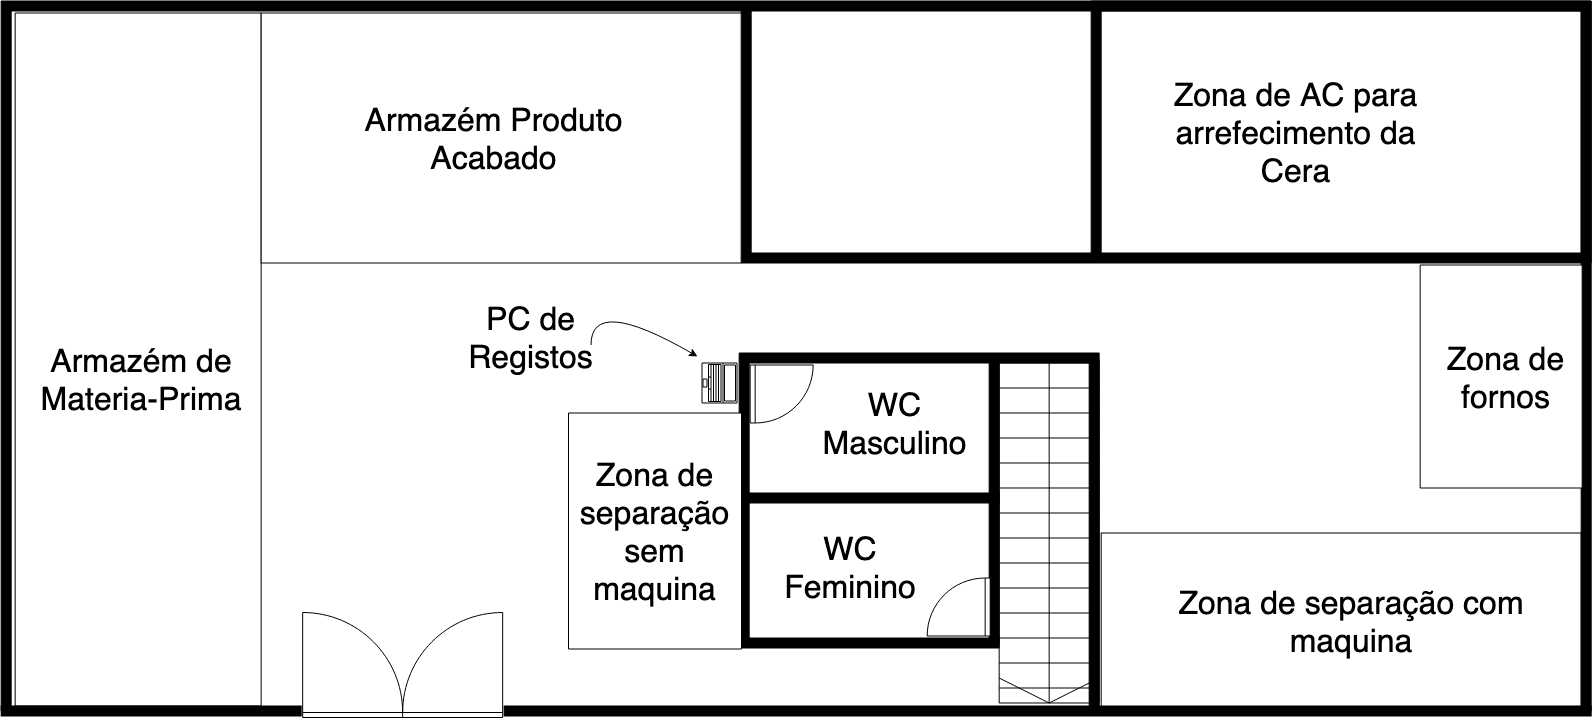
\includegraphics[width=\textwidth,keepaspectratio]{figuras/PlantaNaturalLife.png}
%		\caption{Planta da fábrica}\label{fig:planta_naturallife} 
%	\end{center}
%\end{figure}

\section{O Problema}
A recolha da informação era feito por meio de uma base de dados desenvolvida com o software Microsoft Access\label{sym:MS_ACCESS} com auxilio de alguns formulários embutidos na mesma. Aquilo que se previa ser uma solução temporária, acabou por se tornar definitiva pela simplicidade que a interface oferecia aos utilizadores, pela simples integração com outras aplicações Microsoft, como o Microsoft Excel\label{sym:MS_EXCEL} e Microsoft PowerBI\label{sym:MS_POWERBI}, e pela dificuldade de encontrar um sistema ERP\label{sym:ERP} comercial com as características da solução temporária, com um custo de aquisição que a empresa pudesse comportar e permitisse obter interfaces simplistas para os utilizadores que já se tinham acostumado com os formulários em Access.
No entanto a solução desenvolvida no Microsoft Access é bastante limitada no que toca a executar o mesmo ficheiro em dois computadores ao mesmo tempo, o que limitava as opções da administração nos seus planos expansão da fábrica ou até fazer gestão da própria empresa durante o período laboral da empresa. Este constrangimento obriga os colaboradores a deslocar-se vários metros até ao único computador da fábrica, onde a base de dados estava, para aí fazerem registos. Por fim esta base de dados não suporta níveis de acesso, o que quer dizer que qualquer pessoa com acesso ao computador poderá não só ver todos os registos da empresa como modificá-los ou até mesmo elimina-los. Assim, pretende-se com este projeto de estágio, a implementação de um novo sistema de recolha e consulta de informação, desenvolvido pelo aluno e consequente migração dos dados anteriormente registados.

\section{Estado da arte}
Existem varias ferramentas para fazer a gestão dos recursos de uma empresa e cada uma com as suas características. Para analisar as opções disponíveis, selecionou-se algumas aplicações ERP de forma a poder comparar os seus recursos com as necessidades da empresa.

\subsection{SAP ERP}
O SAP ERP é o produto principal da empresa alemã SAP AG, líder no segmento de software corporativos.\cite{Wikipediab}. O SAP ERP é um sistema integrado de gestão empresarial transacional composto por vários tipos de módulos, cada um responsável por uma parte da atividade da empresa.


\subsection{Primavera Executive}
O PRIMAVERA Executive é um software ERP desenvolvido pela empresa PRIMAVERA Business Software Solutions com foco nas pequenas e médias empresas \cite{PRIMAVERABSS}. A PRIMAVERA Business Software Solutions é uma empresa que se dedica ao desenvolvimento e comercialização de soluções de gestão e plataformas para integração de processos empresariais \cite{Wikipediaa}. Esta empresa afirmou-se no mercado nacional de soluções informáticas de gestão por ser pioneira no desenvolvimento de aplicações para Windows. \cite{Wikipediaa}.
Esta solução inclui ainda integração com os softwares de faturação PRIMAVERA.

\subsection{Microsoft Dynamics}
Microsoft Dynamics é um pacote software da Microsoft destinado a gestão corporativa ERP, para ajudar na tomada de decisões gerenciais e melhorar os resultados administrativos e financeiros das empresas.\cite{Wikipediac}
Dentro deste pacote de software existem as seguintes aplicações:
\begin{itemize}
	\item Dynamics 365 for Sales
	\item Dynamics 365 for Retail
	\item Dynamics 365 for Finance and Operations
	\item Dynamics 365 for Talent
\end{itemize}
Este pacote está disponível em várias edições nas quais varia as funcionalidades disponíveis de modo a se ajustar melhor às necessidades da empresa.

\newpage

\section{Comparação das opções disponíveis}
A informação coletada sobre as diferentes opções foi colocada na tabela \ref{tab:opcoes_mercado}

\begin{longtable}{|m{0.30\textwidth}|m{0.10\textwidth}|m{0.10\textwidth}|m{0.10\textwidth}|m{0.20\textwidth}|}
	\hline
	Característica & SAP & \specialcell{Primavera\\Executive} & \specialcell{Microsoft\\Dynamics} & Solução Própria\\ \hline
	Funções de gestão 
	de recursos da empresa		& \ding{51} & \ding{51} & \ding{51} & \ding{51}\\ \hline
	Acesso remoto externo		& \ding{51} & \ding{51} & \ding{51} & \ding{53}\\ \hline
	Suporte técnico de terceiros& \ding{51} & \ding{51} & \ding{51} & \ding{53}\\ \hline
	Controlo do desenvolvimento & \ding{53} & \ding{53} & \ding{53} & \ding{51}\\ \hline
	Atualizações do sistema		& \ding{51} & \ding{51} & \ding{51} & tem de as
																	desenvolver\\ \hline
	Adaptação total do sistema
	às necessidades da empresa	& \ding{53} & \ding{53} & \ding{53} & \ding{51}\\ \hline
	Implementação apenas dos recursos necessário
								& \ding{53} & \ding{53} & \ding{53} & \ding{51}\\ \hline
	Compatível com os planos de investimento a curto e médio prazo
								& \ding{53} & \ding{53} & \ding{53} & \ding{51}\\ \hline
	Curto período de adaptação dos utilizadores ao novo sistema
								& \ding{53} & \ding{53} & \ding{53} & \ding{51}\\ \hline
	\caption{Tabela resumo das opções de sistemas já desenvolvidos}
	\label{tab:opcoes_mercado}
\end{longtable}

\section{Opção escolhida}
No final desta analise, o caminho definido pela administração da Natural Life para o projeto foi a criação de uma nova plataforma, sendo que essa era a intenção da empresa desde o incio. Por esse motivo foi feita uma nova analise de opções à cerca do desenvolvimento da plataforma. Este documento foi entregue à administração para que o analisa-se o decidisse o modo como a aplicação deveria ser desenvolvida. O documento entregue esta presente no \hyperref[anexo:A]{Anexo A}. Desse documento é possível extrair a tabela comparativa com as diferentes opções para o desenvolvimento da plataforma. Essa tabela é apresentada na tabela \ref{tab:opcoes_dev}.


\begin{longtable}{|p{0.20\textwidth}|p{0.15\textwidth}|p{0.25\textwidth}|p{0.25\textwidth}|}
	\hline
	& Opção                                                 & Vantagens                                                           & Desvantagens                                                                                        \\ \hline
	\multirow{6}{*}{Tipo de Aplicação}                                      & \multirow{3}{*}{Desktop}                              &                                                                     & Necessidade de configurar cada computador que receber a aplicação                                   \\
	&                                                       &                                                                     & Parar o computador para atualizar a aplicação                                                       \\
	&                                                       &                                                                     & Necessidade de um servidor de base de dados                                                         \\ \cline{2-4}
	& \multirow{3}{*}{Web}                                  & Acesso direto em qualquer computador                                & Necessidade de um servidor web e de base de dados                                                   \\
	&                                                       & Maior familiaridade com a plataforma por parte de programador       &                                                                                                     \\
	&                                                       & Menos pontos de falha                                               &                                                                                                     \\ \hline
	
	\multirow{5}{*}{Sistema Operativo}                                      & \multirow{3}{*}{Windows 10}                           & Familiaridade com o sistema                                         & Necessidade de comprar uma licença do Windows Server                                                \\
	&                                                       & Todas as máquinas já executam esta plataforma                       & Necessidade de aprender ASP.NET ou usar o XAMPP                                                     \\
	&                                                       &                                                                     & Se não for usado só software Microsoft não há garantias de segurança/ compatibilidade com o Windows \\ \cline{2-4} 
	& \multirow{2}{*}{Ubuntu 18.04}                         & Plataforma líder de mercado                                         & Curva de aprendizagem para manutenção básica                                                        \\
	&                                                       & Milhares de pacotes no repositório que são revisados pela Canonical &                                                                                                     \\ \hline
	
	\multirow{10}{*}{\specialcell{Sistema de Gestão\\de\\Base de Dados}}    & \multirow{3}{*}{\specialcell{Microsoft SQL\\Server}}  & Familiaridade com o software                                        & Versão Express limitada.                                                                            \\
	&                                                       & Versão Express gratuita                                             & Versões Enterprise e Standard pagas                                                                 \\
	&                                                       &                                                                     & Versão Developer não utilizável em produção                                                         \\ \cline{2-4}
	& \multirow{7}{*}{MariaDB}                              & Gratuito (versão Open Source)                                       & Não possui um ficheiro único para a base de dados.                                                  \\
	&                                                       & Totalmente compatível com MySQL da Oracle                           & Tem de ser instalado manualmente no Windows ou usado com recurso ao XAMPP                           \\
	&                                                       & Padrão no Ubuntu e no XAMPP                                         &                                                                                                     \\
	&                                                       & Escalável                                                           &                                                                                                     \\
	&                                                       & Fiável                                                              &                                                                                                     \\
	&                                                       & Recursos semelhante ao MS SQL Server                                &                                                                                                     \\
	&                                                       & Suporte nativo no Ubuntu                                            &                                                                                                     \\ \hline
	
	\multirow{5}{*}{Tipo de Máquina}                                        & \multirow{2}{*}{Real}                                 & Não dependência da operação de outras máquinas                      & Hardware dedicado                                                                                   \\
	&                                                       &                                                                     &                                                                                                     \\ \cline{2-4}
	& \multirow{3}{*}{Virtual}                              & Não necessita de hardware dedicado.                                 & Exige que o utilizador que esta a executar a VM nunca termine a sessão.                             \\
	&                                                       & Várias instâncias da máquina ao mesmo tempo.                        & Se a máquina real tiver de ser reiniciada, a VM tem de ser interrompida                             \\
	&                                                       & Backup muito fácil.                                                 & Partilha dos recursos da máquina hospedeira com a maquina virtual.                                  \\
	\hline
	\caption{Tabela resumo das opções para o desenvolvimento}
	\label{tab:opcoes_dev}
\end{longtable}



\section{Analise das opções disponíveis para o desenvolvimento do projeto}
O documento entregue incide sobre os aspetos base para a criação do sistema de informação: tipologia de aplicação, servidor, sistema de gestão de base de dados, linguagens de programação.

O primeiro a ser definido seria o tipologia de aplicação. Decidir sobre uma aplicação web ou uma plicação desktop poderia condicionar o trabalho futuro. Aqui a sugestão passou pelo desenvolvimento de uma aplicação web, pois esta seria agnóstica de equipamento o que dava uma grande flexibilidade no futuro. Além deste fator, já se sabia que teria de existir uma máquina servidor pois teria de haver uma base de dados centralizada, logo não havia nenhum gasto extra com esta solução. Esta sugestão acabou por ser aceite, em conjunto com as linguagens de programação PHP para o back-end e JavaScript para o front-end. Ficou ainda decidido que de modo a tornar o desenvolvimento mais ágil e dar robustez ao serviço, devia ser utilizado o framework Laravel. Esta escolha assentou no facto deste framework já ser bastante utilizado e testado ao redor do mundo. Inclusive é tido como escolha de referencia para projetos de missão crítica em PHP pelas suas características de segurança\cite{Mansuri2018}.

Segundo ponto a ser definido foi o sistema de gestão de base de dados. Apesar das vantagens enunciadas em relação ao MariaDB, a opção opção recaiu sobre o Microsoft SQL Server. Quanto ao sistema operativo do servidor a opção tomada foi o Ubuntu Server 18.04 em maquina física, pois havia a intenção por parte da administração em separar o servidor de qualquer outra máquina já existente.
Um tópico que não foi considerado neste documento foi o sistema e serviço de versionamento. A administração optou por deixar à escolha do estudante desde que o houvesse a garantia de o repositório ser um repositório privado, uma vez que tirando o facto de ser um repositório privado, esta opção em nada influenciava o sistema a ser implementado. Assim o sistema de versionamento escolhido foi o Git no serviço GitHub.

\section{Resumo final das opções tomadas para o desenvolvimento do projeto}
Construir uma plataforma própria em formato de aplicação Web. Esta aplicação web seria construida em PHP, com o framework Laravel, para o backend e JavaScript frontend. O sistema de gestão de base de dados escolhido foi o Microsoft SQL Server na edição Express e o servidor seria uma máquina física com o sistema operativo Ubuntu 18.04. Para fazer o versionamento do código foi utilizado um repositório privado no serviço GitHub.